\documentclass[12pt]{article}
\usepackage[letterpaper]{geometry}
\geometry{top=1.0in, bottom=1.0in, left=1.0in, right=1.0in}
%\usepackage[margin=.9in]{geometry}
%\usepackage{probstat}
\usepackage{amsfonts}
\usepackage{hyperref}
\usepackage{setspace}
%\usepackage{Sweave}
\usepackage{algorithm2e}
\setstretch{1} 

\makeatletter
\renewcommand\section{\@startsection{section}{1}{\z@}%
                                  {-3.5ex \@plus -1ex \@minus -.2ex}%
                                  {2.3ex \@plus.2ex}%
                                  {\normalfont\large\bfseries}}
\makeatother

%\setlength{\parindent}{1cm}
\usepackage[utf8]{inputenc}
\usepackage[nogin]{Sweave}
\usepackage{amsthm}
\usepackage{fancyhdr}
\usepackage{times}
\fancyhf{}
\renewcommand{\headrulewidth}{0pt} 
\renewcommand{\footrulewidth}{0pt} 
\setlength\headsep{0.333in}
%\setlength{\parindent}{1cm}
\newcommand{\bibent}{\noindent \hangindent 40pt}
%\newcommand{\par}{\indent}
\newenvironment{workscited}{\newpage \begin{center} \large{\textbf{Works Cited}} \end{center}}{\newpage }
\newtheorem{Lorenz}{Definition}
\newtheorem*{Gini}{Hurdle Rule}
\newtheorem{LL}{Theorem}
\newtheorem{mvt}[LL]{Theorem}
\newtheorem{density}[LL]{Theorem}
\newtheorem{densitya}[LL]{Theorem}
\newtheorem{cdf}[LL]{Theorem}
\newtheorem{ftpdensity}[LL]{Theorem}
%%%%% edit the next few lines using your information
%
\chead{}
\lhead{Daniel Stahl}
\rhead{\thepage}
\title{Distribution of First Hitting Time}
\pagestyle{fancy}


\def\R{{\sf R}}
\def\Rstudio{{\sf R}Studio}

%%%% some things to improve how R output looks


\def\myRuleColor{\color{black!50!white}}


\fvset{listparameters={\setlength{\topsep}{0pt}}} 
\renewenvironment{Schunk}{\vspace{\topsep}}{\vspace{\topsep}} 



\begin{document}
\Sconcordance{concordance:distributionTau.tex:distributionTau.Rnw:%
1 76 1 1 20 84 1 1 96 1 35 2 1 1 20 1 3 3 1 1 11 1 2 2 1 1 12 1 2 1 1}

\setlength{\parindent}{0pt}
%\parindent=0pt
%\parskip=3mm


%%%% some set-up for Sweave









%%% R stuff to execute at the beginning of the document.
%%% Note: even default packages need to be required here.

%%%%%% main content goes below here
%\pagestyle{empty}
\maketitle
\section{Introduction}

\section{Derivation for the Laplace transform of first hitting time for GBM}

Let \(dS=\alpha S dt+\sigma S dW_t\) and \(\tau\) be a stopping time such that \(S_\tau=m\).  By Dynkan's formula, 

\[\mathbb{E} [e^{-u\tau}f(S_\tau)]=f(S_0)+\mathbb{E}\left[ \int_0  ^ \tau \left(f_{S} \alpha S + \frac{1}{2} f_{SS} \sigma^2 S^2-uf\right) e^{-us} ds\right]\]

If \(f(x)\) satisfies 

\[f_x \alpha x+\frac{1}{2} f_{xx} \sigma^2 x^2 -uf=0\]

Then Dynkan's formula implies that 

\[\mathbb{E}[e^{-u\tau} f(S_\tau)]=f(S_0)\]

If \(f(S_\tau)=1\) and \(f(0)=0\) then \(f\) is uniquely determined and is the Laplace transform of the density of \(\tau\).  It remains only to solve the ODE.  Introducing \(\gamma_+\) and \(\gamma_{-}\) where \[\gamma =  \left(\frac{\sigma^2}{2}-\alpha  \pm \sqrt{\left(\alpha -\frac{\sigma^2}{2}\right)^2+2u\sigma^2}\right)/\sigma^2\]
The solution can be written as \(c_1 S ^ {\gamma_+}+c_2 S^{\gamma_{-}}\).   If \(S<m\) then \(c_2\) must be zero or \(f\) tends towards positive or negative infinity as \(S \to 0\).  On the other hand, if \(S>m\) then \(c_1\) must be zero or \(f\) tends towards positive or negative infinity as \(S \to \infty\).  Therefore the solution to the ODE is as follows (making explicit the dependence on \(u\)):

\begin{equation}
f(u; S)=\left\{
\begin{array}{rl}
\left(\frac{S}{m} \right) ^ {\gamma_{+}} , & \mathrm{if}  S<m \\
\left(\frac{S}{m} \right) ^ {\gamma_{-}}, & \mathrm{if} S>m
\end{array}
\right.
\end{equation}

\section{Characteristic function of general diffusion}

Consider a diffusion satisfying
\[dX=\alpha(X, t)dt+\sigma(X, t)dW_t\]

Then the solution of the ODE 

\[f_x \alpha(X, t)+ \frac{\sigma^2}{2}f_{xx} dt- uif=0\]

is the characteristic function of \(\tau\).  The distribution can then be recovered using inversion techniques.  However, the ODE tends not to have analytical solutions, being non-linear and second order.  

\subsection{Numerical algorithm}

Discretizing the ODE and solving it numerically is has linear complexity.  Solving the ODE in this way yields the approximate solution for \(x \in (0, m)\), but only for a single value of \(u\).  Therefore the ODE must be solved multiple times in order to obtain the characeteristic function for each discretized \(u\).  Fortunately once the matrix of values is obtained the density function can be recovered for each discretized \(x \in (0, m)\).

The total complexity for computing the matrix is \(O(l*n)\)


\section{Characteristic Function Algorithms}
Let g(x) be the density function of \(\tau\).  By Fourier's theorem, 
\[g(x)=\frac{1}{2\pi} \int e^{iux} f(u) du \]


\subsection{Cosine Method}
Oosterlee  and Fang (2008) proposed a novel method to price European options for a very diverse set of asset models.  This method relies on inverting the characteristic function of the underlying log price; and prices options with many strikes simultaneously.  Along the way they demonstrated the surprising accuracy of the method in computing the probability density from the characteristic function.  Since the authors' main goal was to price options they spent minimal time on this result. Two key characteristics of this algorithm are the separate computations of the \(x\) and \(u\) domains and the exponential convergence of the algorithm.  The method that the authors devised only requires \(O(nlk)\) operations to compute the density where \(k\) is the number of steps in the \(x\) domain and due to the excellent convergence properties \(m\) does not typically have to be larger than \(128\).  




The following plot shows the actual pdf (red), the inverted analytical characteristic function (blue), and the numerically solved ODE for the characteristic function that is then inverted (black).  The parameters are \(m=5, s=1, sigma=.3, alpha=.1, n=512, k=1024, l=200\).

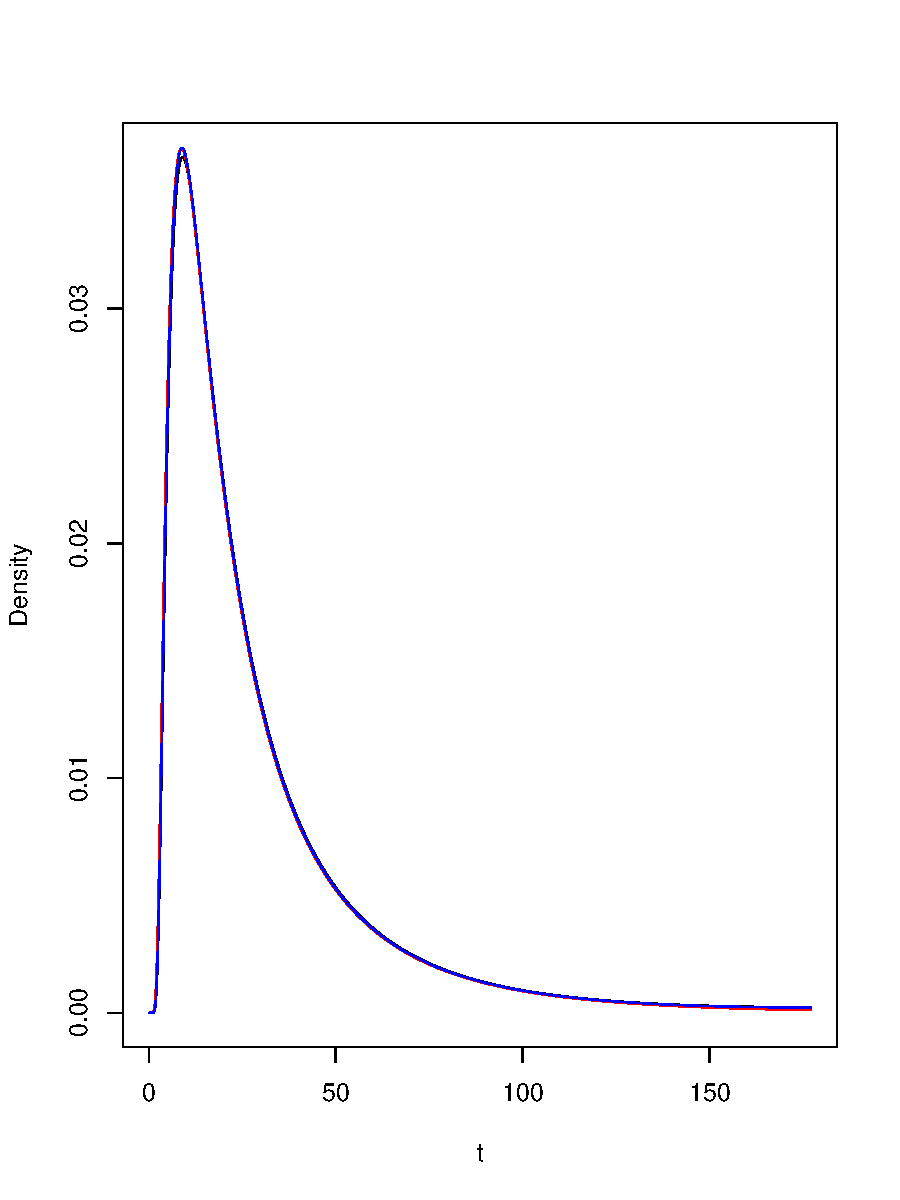
\includegraphics{fig-006}

The next plot is based off the CEV model with \(\delta=.8\).  Having no analytical solution to either the characteristic function or the density, only the numerical ODE solution is presented.  The density of the distribution when \(\delta=1\) is presented to show the effect that \(\delta\) has on the distribution of the first hitting time.


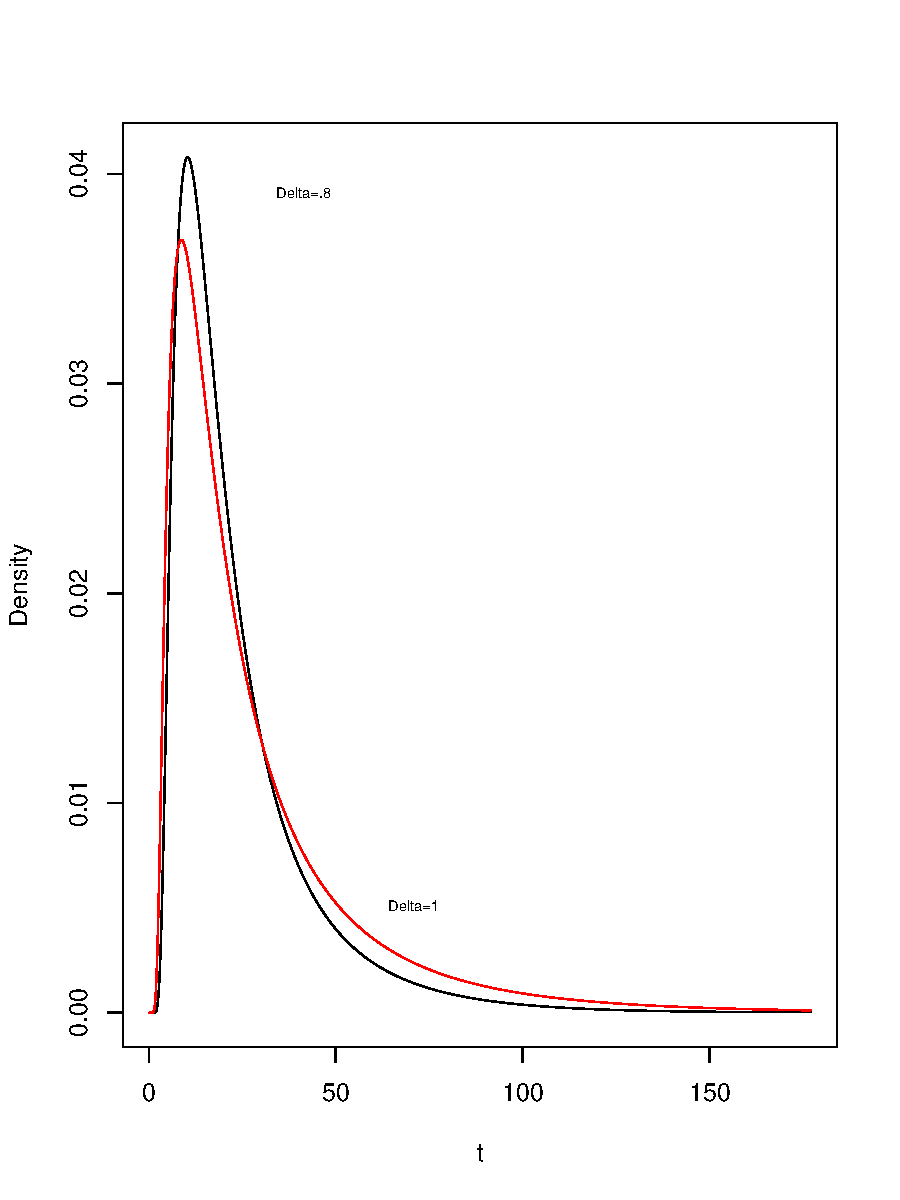
\includegraphics{fig-007}

Since the algorithm computes the density for every node on the ODE, the following is the pdf for several values of \(S\).

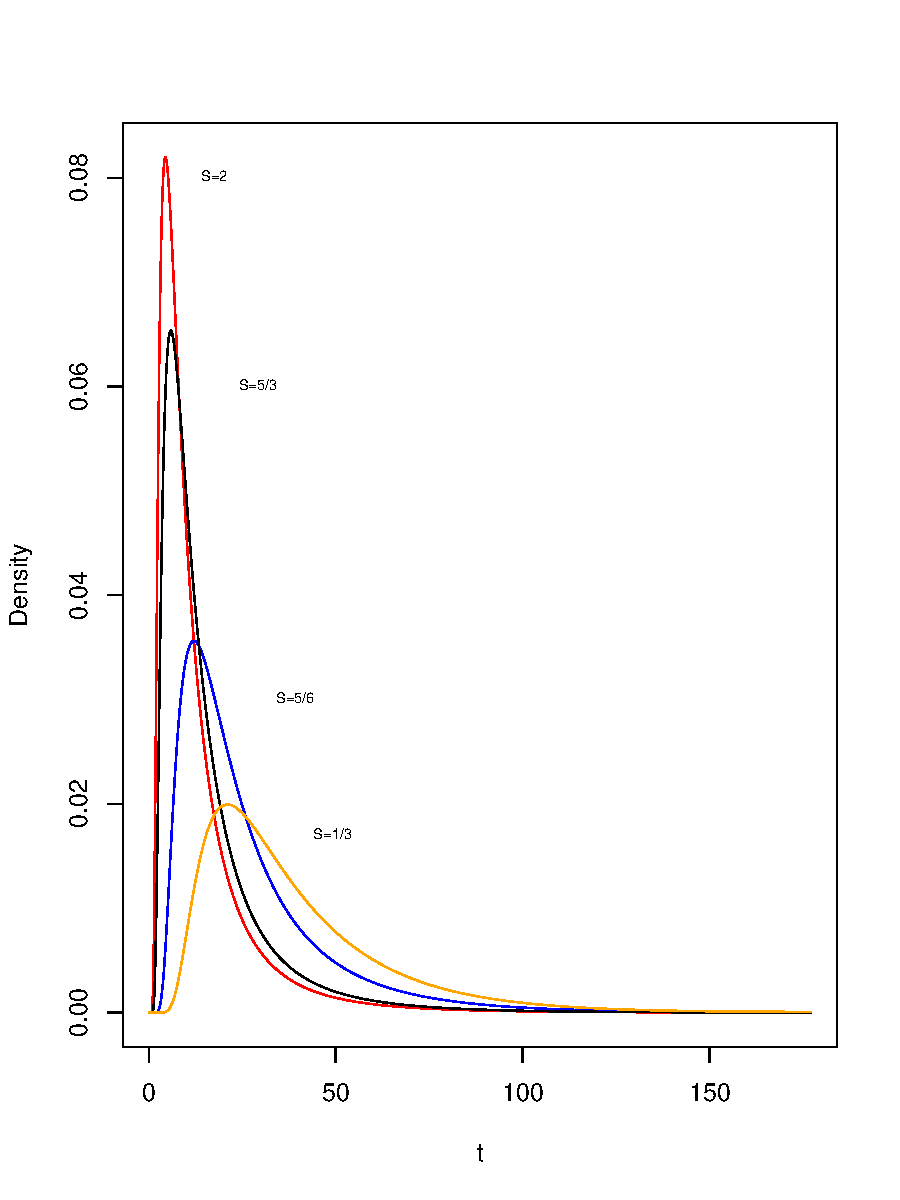
\includegraphics{fig-008}

\end{document}
